\documentclass[main.tex]{subfiles}
\begin{document}

\begin{flushleft}
\Large{\bf{Literature Survey}}
\end{flushleft}
\vspace{1.5mm}
\begin{flushleft}
\bf{Paper 1: Diagonal Based Feature Extraction For Handwritten Alphabets 
	Recognition System Using Neural Network}
\end{flushleft}
\vspace{1.5mm}
\justify
In this paper, a diagonal feature extraction scheme for recognizing offline
handwritten characters is proposed. In the feature extraction process, resized
individual character of size 90 * 60 pixels is further divided into 54 equal
zones, each of size 10 * 10 pixels. The features are extracted from the pixels
of each zone by moving along their diagonals. This procedure is repeated for all
the zones leading to extraction of 54 features for each character. These
extracted features are used to train a feed forward back propagation neural
network employed for performing classification and recognition tasks. Extensive
simulation studies show that the recognition system using the diagonal features
provides good recognition accuracy while requiring less time for training. The
proposed recognition systems is given by-
\begin{figure}[H]
	\centering
	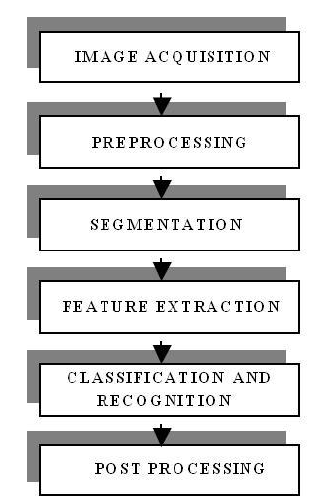
\includegraphics{figures/figure-1.png}
	\caption{Schematic diagram of the proposed recognition system}
	\label{fig1}
\end{figure}
Pre-processing consists of performing subtasks of noise removal, binarization,
edge detection and dilation and filling on the scanned input image to further
provide it to the feature extraction block. In the segmentation stage, an image
of sequence of characters is decomposed into sub-images of individual character.
The isolated characters are assigned a number for each distinct character as
part of the labelling process. The labelling provides information about the
number of characters in the image. Each individual character is uniformly
resized into 90 * 60 pixels for classification and recognition stage. Then comes
the diagonal feature extraction scheme as mentioned above. The features are
extracted from each zone pixels by moving along the diagonals of its respective
10 * 10 pixels. Each zone has 19 diagonal lines and the foreground pixels
present long each diagonal line is summed to get a single sub-featurem thus 19
sub-features are obtained from each zone. These 19 sub-features are averaged to
form a single feature value and placed in the cooresponding zone. This procedure
is sequentially repeated for all the zones. There could be some zones whose
diagonals are empty of foreground pixels. The feature values corresponding to
these zones are zero. Finally, 54 features are extracted for each character. In
addition, 9 and 6 features are obtained by averaging the values placed in zones
rowwise and columnwise, respectively. As result, every character is represented
by 69, that is, 54 + 15 features. The classification stage is the decision
making part of a recognition system and it uses the features extracted in the
previous stage. A feed forward back propagation neural network having two hidden
layers with architecture 54-100-100-38 is used to perform the classification.
The hidden layers use the log sigmoid activation function, and the output layer
is a competitive layer, as one of the characters is to be identified. The number
of neurons in the hidden layers is chosen by trial and error. The neural network
specifics are given by-
\begin{center}
\begin{itemize}
	\item Input nodes : 54 / 69
	\item Hidden nodes : 100 each
	\item Output nodes : 38 (26 alphabets, 10 numerals and 2 special symbols)
	\item Training algorithm : Gradient descent with momentum training and
		adaptive learning
	\item Perform function : Mean square error
	\item Training goal achieved : 0.000001
	\item Training epochs : 1000000
	\item Training momentum constant : 0.9
\end{itemize}
\end{center}
The comparison of recognition rate results obtained using different orientations
with 54 features is given by-
\begin{center}
	\begin{tabular}{|c|c|c|c|}
\hline
Networks & 1 & 2 & 3 \\
\hline
Feature Extraction type & Vertical & Horizontal & Diagonal \\
\hline
Number of nodes in input layer & 54 & 54 & 54 \\
\hline
Number of nodes in 1st hidden layer & 100 & 100 & 100 \\
\hline
Number of nodes in 2nd hidden layer & 100 & 100 & 100 \\
\hline
Number of nodes in output layer & 26 & 26 & 26 \\
\hline
Recognition rate percentage & 92.69 & 93.68 & 97.80 \\
\hline
\end{tabular}
\end{center}
\vspace{5mm}
\begin{flushleft}
\bf{Paper 2: An Overview Of Character Recognition Focused On Off-line
	Handwriting}
\end{flushleft}
\vspace{1.5mm}
This paper focuses on the methodologies of CR systems, emphasizing the offline
handwriting recognition problem. A heirarchical approach for most of the systems
is given by \textbf{\textit{pixel - feature - character - sub-word - word -
meaningful text}}. The paper gives an overall idea, a summary of various methods
which can be used to perform various tasks present in the complete process of
handwriting recognition. The pre-processing stage consists of noise reduction via
filtering, morphological operations and noise modeling, normalization  of the
data via skew normalization and baseline extraction, slant normalization, size
normalization and contour smoothing, compression in the amount of information to
be retained via thresholding and thinning. The segmentation phase consists of
external and internal segmentation which further consists of explicit and
implicit segmentation and mixed strategies which combine these two techniques.
Represention consists of global transformation and series expansion via fourier
transforms, gabor transform, wavelets, moments and Karhunen-Loeve expansion,
statistical representation via zoning, crossings and distances and projections,
geometrical and topological representation via extraction of counting
topological structures, measuring and approximating the geometrical properties,
coding and graphs and trees. The training and recognition techniques enumerated
are template matching via direct matching, deformable templates and elastic
matching and relaxation matching, statistical techniques like parametric and
non-parametric recognition, clustering analysis, hidden markov modeling and fuzzy
set reasoning, strutural techniques like grammatical and graphical methods, and
finally neural networks. Post processing consists of retaining contextual
information of the entire text and in order to achieve this, a feedback loop is
set up which feeds the information obtained after recognition back to the input
of the system to improve the recognition model by reducing latency and
increasing efficiency. Current studies in CR research is given by-
\begin{figure}[H]
	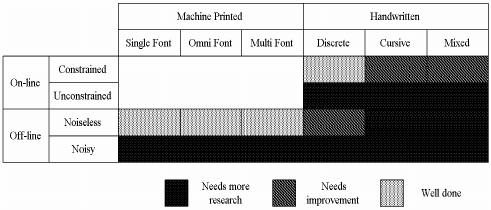
\includegraphics[width=\linewidth]{figures/figure-2.png}
	\caption{Current status of the existing intelligent character recognition
	systems}
	\label{fig2}
\end{figure}
\begin{flushleft}
\bf{Paper 3: An Offline Approach to Handwriting Recognition}
\end{flushleft}
\vspace{1.5mm}
The paper mentions that the central tasks of offline handwriting recognition are
character and word recognition. Document analysis is the necessary preliminary
step in recognition that locates appropriate text when complex, two-dimensional
spatial layouts are employed. According to this paper, pre-processing consists
of thresholding, noise removal, line segmentation and word and character
segmentation. This is given by-
\begin{figure}[H]
	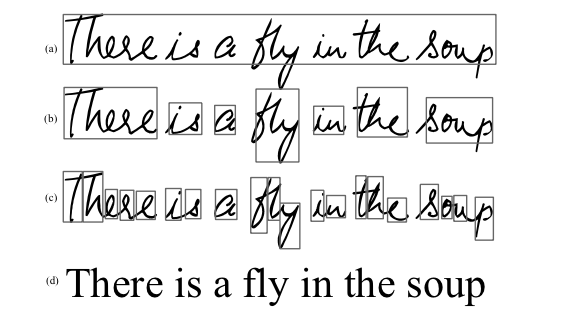
\includegraphics[width=\linewidth]{figures/figure-3.png}
	\caption{Line, word and character segmentation}
	\label{fig3}
\end{figure}
The basic problem of character recognition is to assign the digitized character
to its symbolic class. A pattern recognition algorithm is used to extract
shape features and to assign the observed character to the appropriate class.
Artifical neural networks have emerged as fast methods for implementing
classifiers for OCR. In difficult cases, it becomes necessary to use models to
constrain the choices at the character and word levels. Such models are
essential in handwriting recognition due to the wide variability of hand
printing and cursive script. A word recognition algorithm attempts to associate
the word image to choices in a lexicon. Typically, a ranking is produced. This
is done either by the analytical approach of recognizing the individual
characters or by holistic approach of dealing with the entire word image. The
latter approach is useful in the case of touching printer chacracters and
handwriting. A high level of performance is observed by combining the results of
both approaches. One method of word recognition based on determining pre
segmentation points followed by determining an optimal path through a state
transition diagram. Another approach utilizes the idea of regular and singular
features. Handwriting is regarded as having a regular flow modified by
occasional singular embellishments. A commmon approach is to use a Hidden Markov
Model to structure the entire recognition process. Another method deals with a
limited size dynamic lexicon. Words that are relevant during the recognition
task are not available during training because they belong to an unknown subset
of a very large lexicon. Word images are over segmented such that after the
segmentation process no adjacent characters remain touching. Instead of passing
on combinations of segments to a generic OCR, a lexicon is brought into play
early in the process. A combination of adjacent segments is compared to only
those character choices which are possible at the position in the word being
considered. The approach can be viewed as a process of accounting for all the
segments generated by a given lexicon entry. Lexicon entries are ordered
according to the goodness of the match. This method is given by-
\begin{figure}[H]
	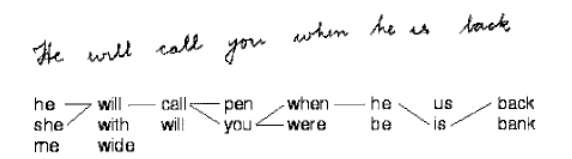
\includegraphics[width=\linewidth]{figures/figure-4.png}
	\caption{Recognition of a line}
	\label{fig4}
\end{figure}
Dynamic programming (DP) is a commonly used paradigm to string the potential
character into word candidates; some methods combine heuristics with DP to
disqualify certain groups of primitive segments from being evaluated if they are
too complex to represent a single character. The DP paradigm also takes into
account compatibility between consecutive character candidates.
\end{document}
\begin{flushleft}
\bf{Paper 4: Offline Handwriting Recognition using Genetic Algorithm}
\end{flushleft}
\vspace{1.5mm}
In this paper, a new method for offline handwriting recognition is presented. A
robust algorithm for handwriting segmentation has been described here with the
help of which individual characters can be segmented from a word selected from a
paragraph of handwritten text image which is given as input to the module. Then
each of the segmented characters are converted into column in the form of text
files. The network has been designed with quadruple layered neural network with
625 input and 26 output neurons each corresponding to a character from a-z, the
outputs of all the four networks is fed into the genetic algorithm which has
been developed using the concepts of correlation, with the help of this the
overall network is optimized with the help of genetic algorithm thus providing
us with recognized outputs with great efficiency of 71\%. The handwriting
recognition model described here works at three stages, segmentation of the
handwritten text, recognition of segmented characters with the help of
artificial neural networks and lastly selecting the best solution from the four
artificial neural network outputs with the help of genetic algorithm.
\par The handwritten document is scanned and taken as an input to obtain 
individual characters which are written in a text file and are later read back 
and are passed as inputs to the four Artificial Neural Networks. In the 
algorithm, the scanned gray scale image is read into an image matrix which is 
converted into a monochromatic image matrix which pixel values of 0 for black 
points and 255 for white points. Then row wise searching is started from the 
point (0,0) to find out the first black point. This is the assumed top point of 
the first word of the handwritten text that has been inputted. This point is 
referred to the “Upper Point”. After the upper point is found, all the black 
pixels that are connected to this pixel are given a value of 999. Once this step
is complete, then all the characters linked to that word have a value of 999
in the matrix under consideration. After finding all the connected points, a row
wise search starts from the bottom to the top to find the first 999 value. This
value corresponds to the “Lowest Point”. After this point is obtained, the area
between the top and bottom point is searched on the left to check if any word 
has been missed on the left. In case another word is present on the left, then 
the new top point is obtained and the bottom point is found again else the 
procedure continues. After this is carried out, the left and right points of the
word are found out by column wise searches. After the four points, the Upper, 
Lower, Right and Left point are found out, the word can be extracted and stored
in a different matrix. This step is followed by marking of intersection points 
between various characters in the cursive handwriting. The word is searched for 
the number of cuts in a column wise manner. All the cases in which number of 
cuts is one and has an edge on either left or its right are marked and then all
the successive markings are averaged to provide one optimum point through which
a cut is marked with gray value of 0.5. After all the cuts are marked, in a loop
all the characters are written into a file which is later read by the neural 
network to recognize the character.
\par The four artificial neural networks used consist of an input layer, three 
hidden layers and an output layer for each of the individual networks. The input
layers takes the input from the image segmentation algorithm thus has 625 input 
neurons. The number of hidden layer neurons is as shown in the Table 1. The 
output layer consists of 26 neurons; this is due to the fact that there are 26 
characters to be identified. Thus each output neuron corresponds to every 
character. Four artificial neural networks have been employed for the character
recognition. The properties of each of the four artificial neural networks are 
designed using different parameters given by-
\begin{figure}[H]
	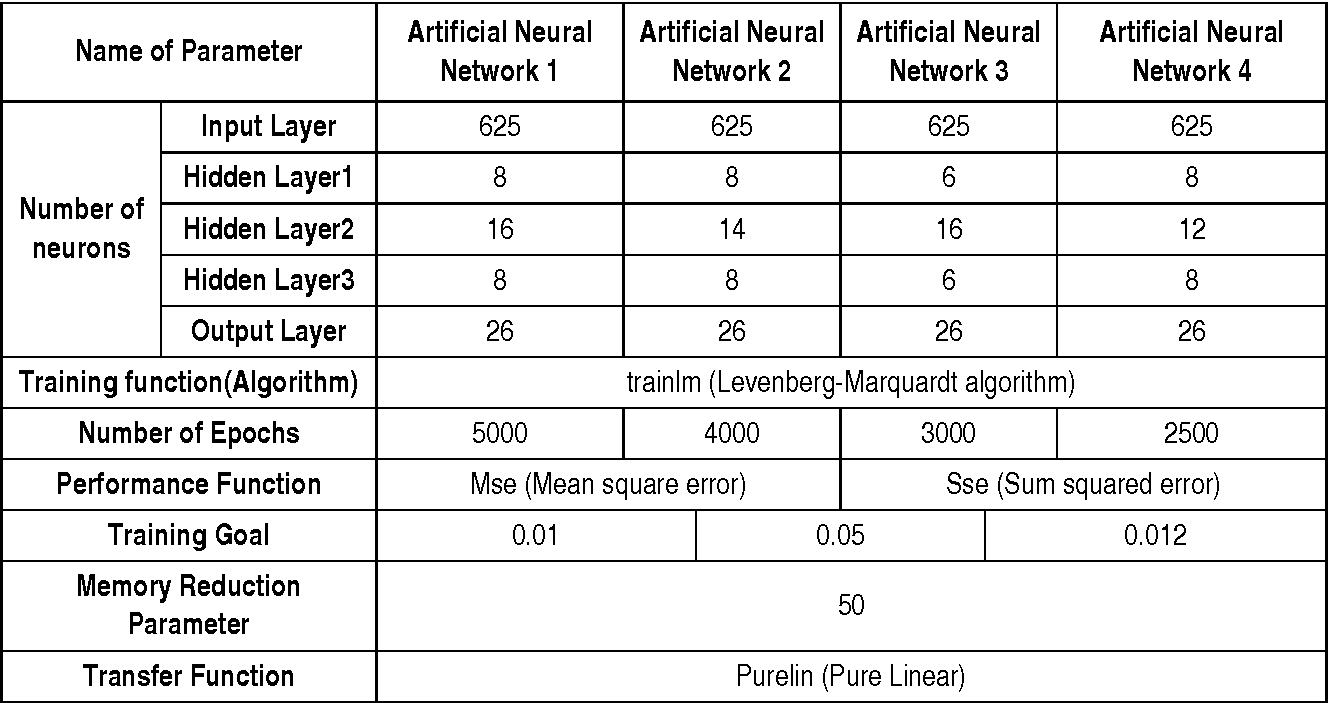
\includegraphics[width=\linewidth]{figures/figure-5.png}
	\caption{List of parameters used for the four artificial neural networks}
	\label{fig5}
\end{figure}
A column vector is generated by the Image Segmentation consisting of 625 
elements, which is saved in a “.txt” file. This “.txt” file is read and the 
elements are fed as an input to each of the four neural networks. These neural 
networks read all the weights and biases values that were saved in another files
during the training process. Corresponding to the input, output is generated at
the output layer. A “1” is set at the index of the characters that has been 
recognized. There can be more than one character that could be recognized based
on the noise in the input of the neural network.
\par The following method is applied genetic algorithm to the outputs of the
four artificial neural networks-
\begin{center}
\begin{enumerate}
	\item \textbf{Initialization} : Select the output of the neural network with
		the indexes comprising of "1's". This corresponds to the initial 
		population for the genetic algorithm.
	\item \textbf{Selection} : Select the indexes from the neural network that 
		has minimum number of "1's".
	\item \textbf{Fitness function} : Compute the correlation coefficients of 
		the selected indexes.
	\item \textbf{Mutation and crossover} : For the correlation coefficients 
		less than the threshold value 0.50 repeat the step of the fitness 
		function for a different training set. Discard the indexes that have 
		coefficient values less than 0.3.
	\item \textbf{Evaluation} : Select the index which has the maximum 
		correlation coefficient with the input matrix.
	\item Output the selected character.
\end{enumerate}
\end{center}
